%\documentclass{article}
%\usepackage{graphicx,subfigure}
%\usepackage{caption,rotating}
%\begin{document}

\begin{figure}[!h]
\centering
\captionsetup{width=0.7\textwidth}
 \subfigure[Sheep 3453 Wrinkled]{
%    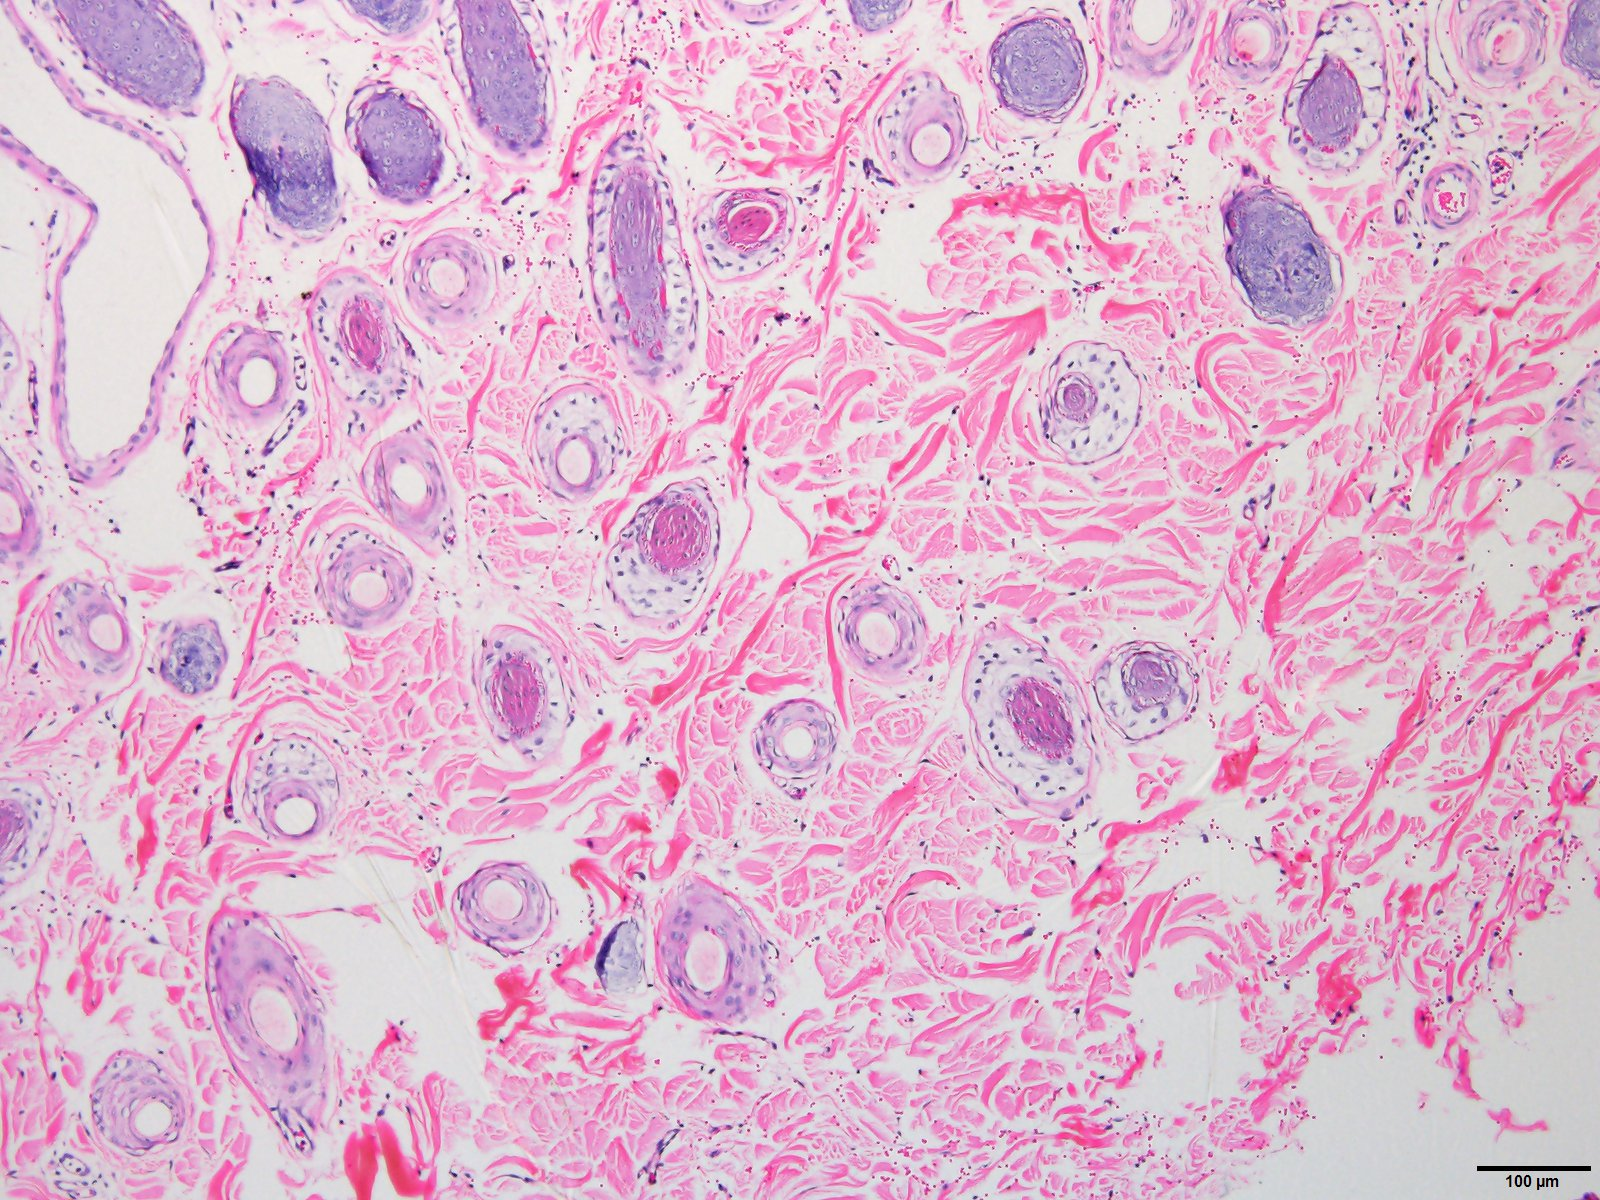
\includegraphics[scale=0.20]{3453_btwn_wrinkle_10x.jpg}
%   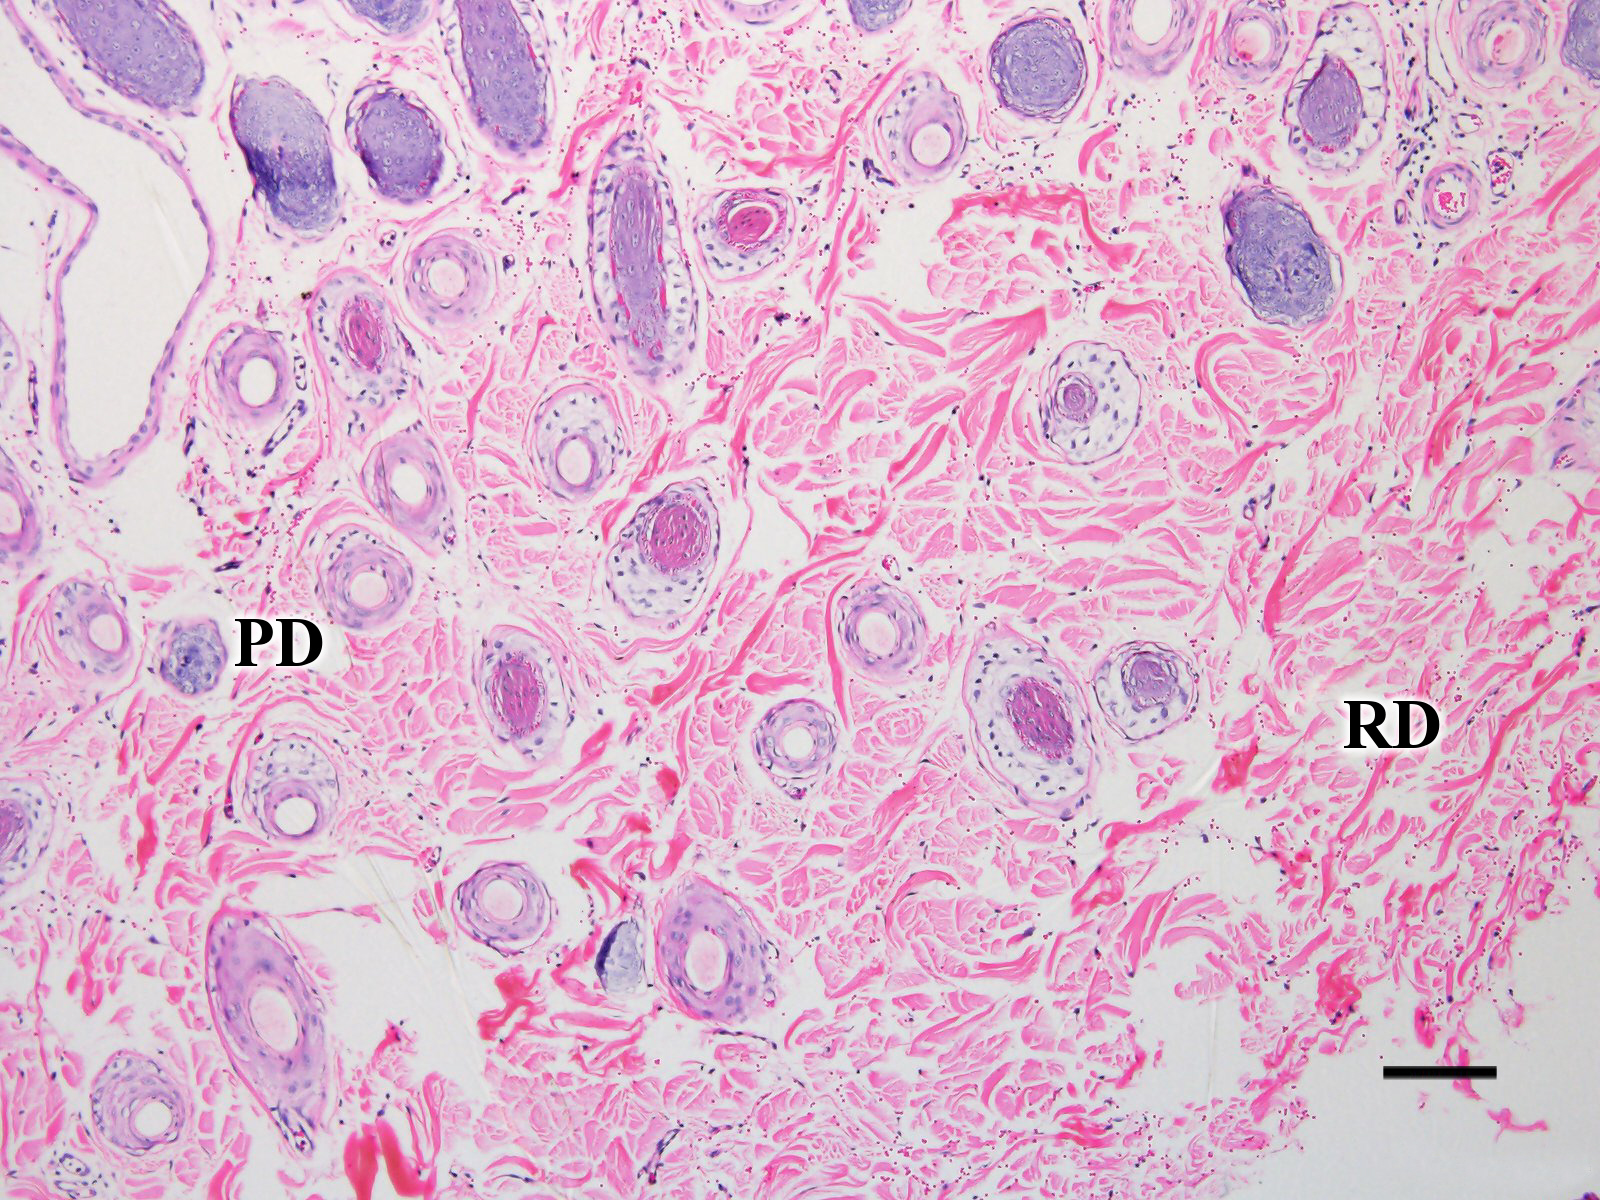
\includegraphics[scale=0.10]{fig8a.jpg}
    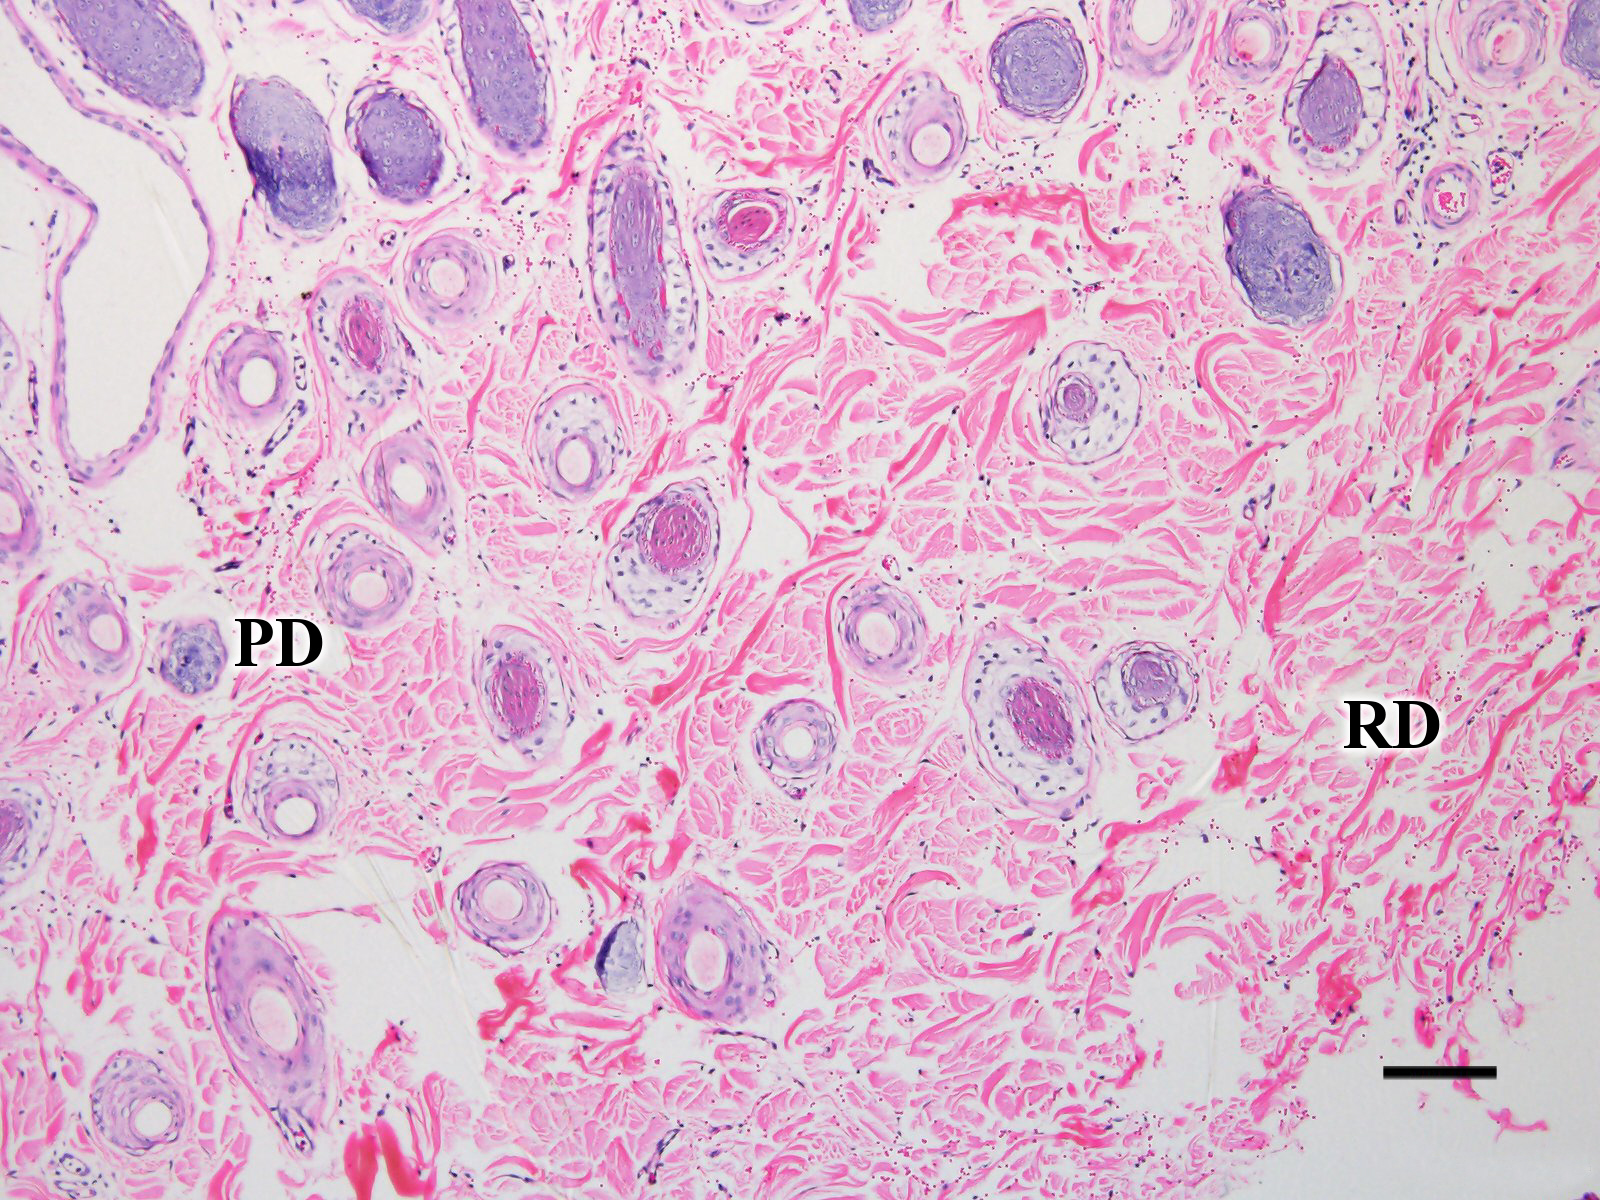
\includegraphics[width=0.7\textwidth]{fig8a.jpg}
% 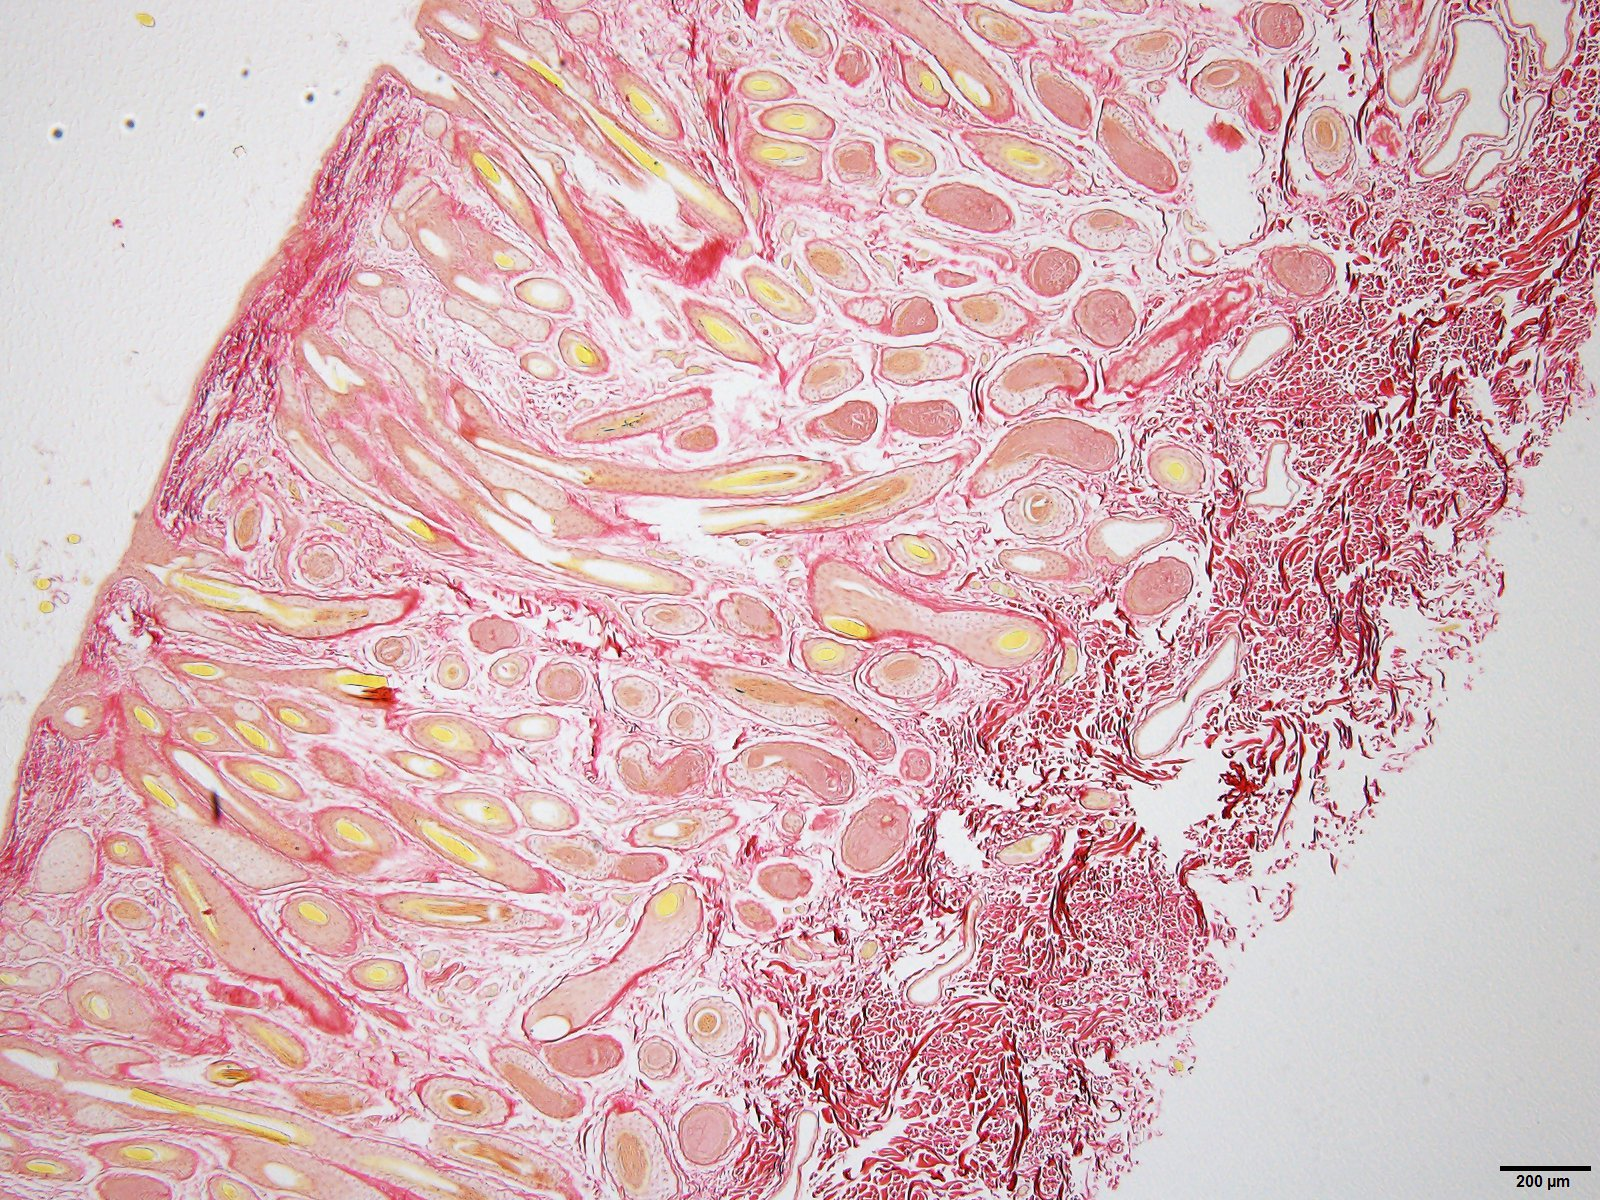
\includegraphics[width=1.0\textwidth]{w479-2-rigid.jpg}
  }
 \subfigure[Sheep 3458 Wrinkle-free]{
%    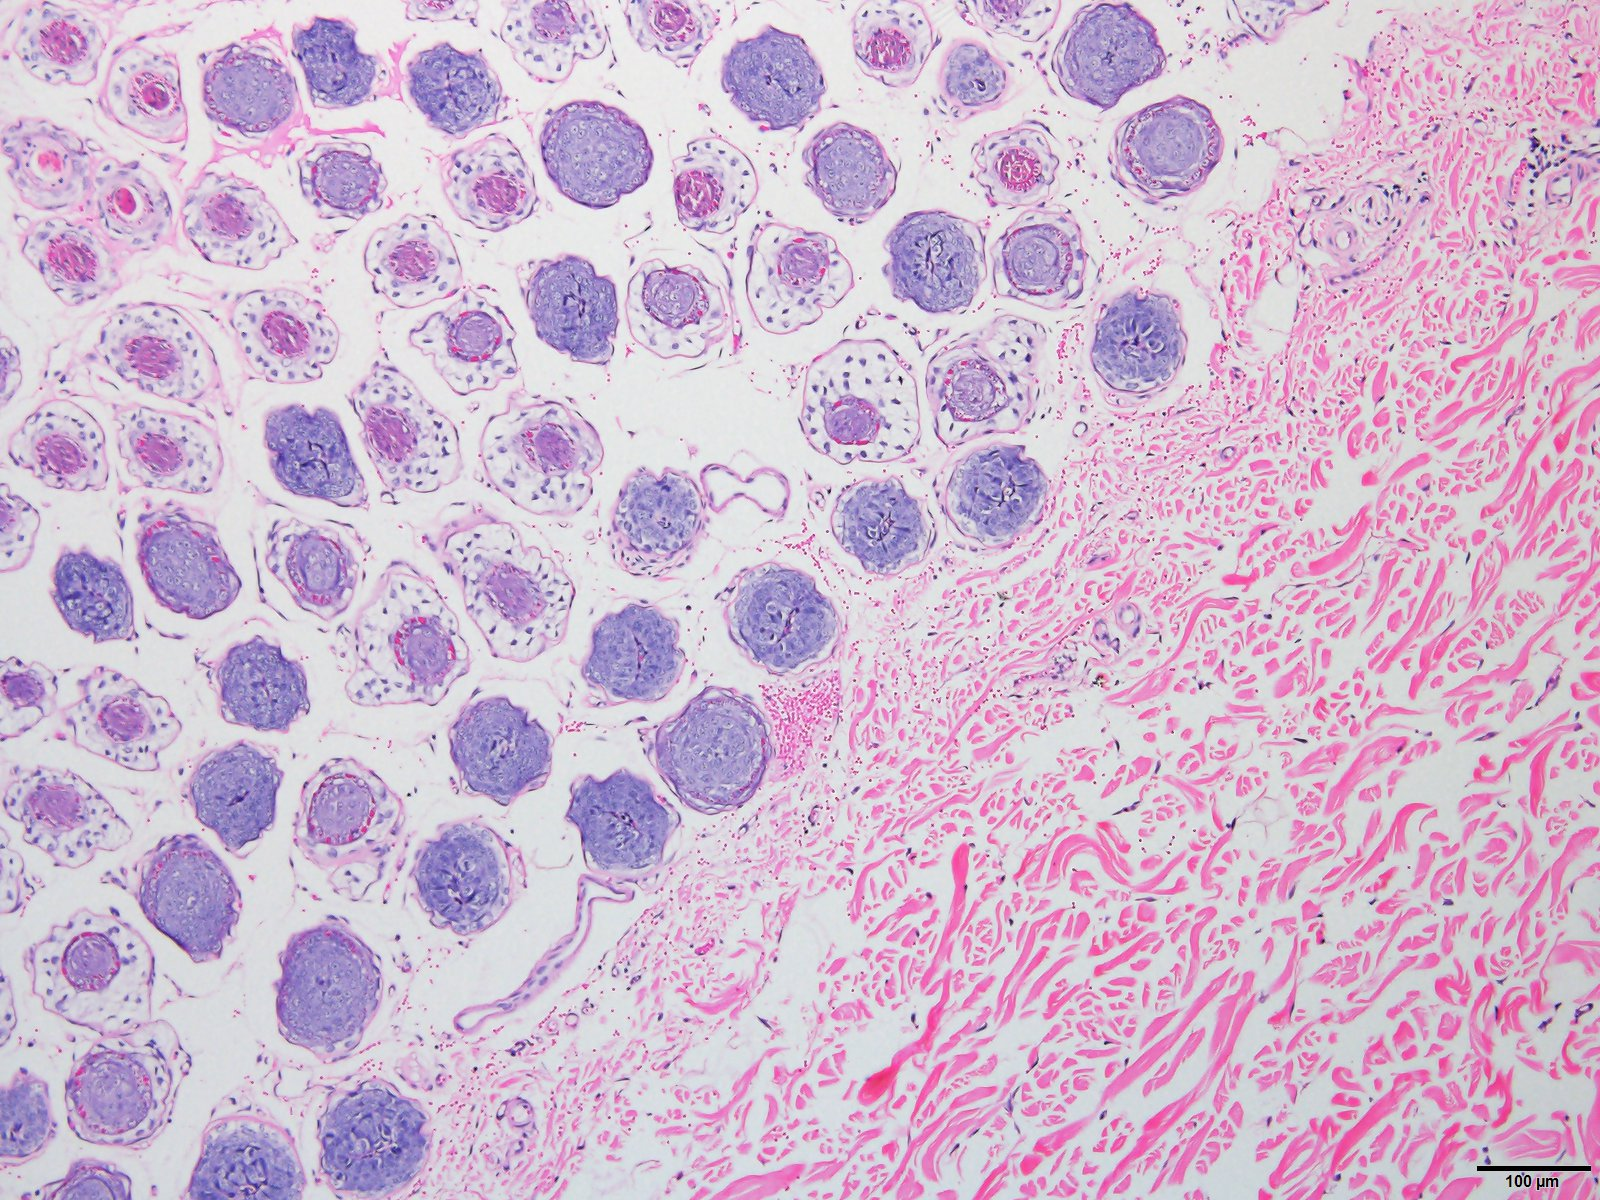
\includegraphics[scale=0.20]{3458_smooth_10x.jpg}
%   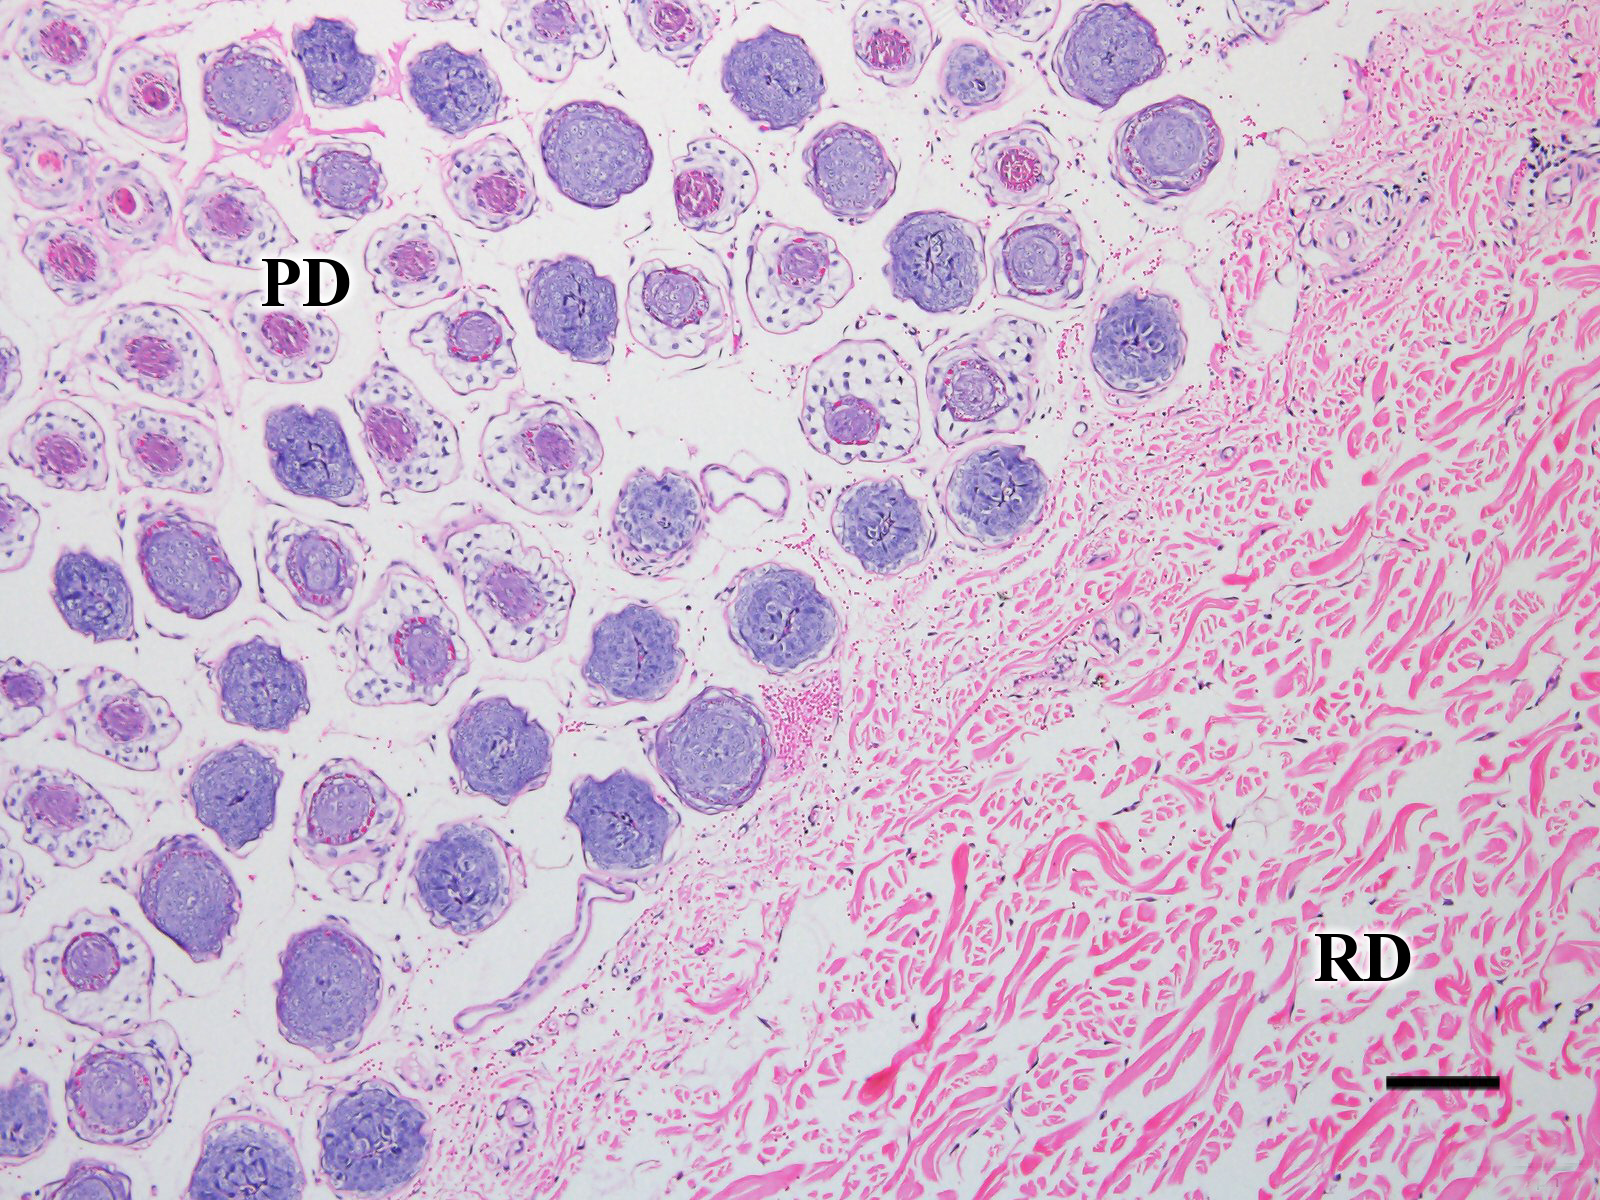
\includegraphics[scale=0.10]{fig8b.jpg}
    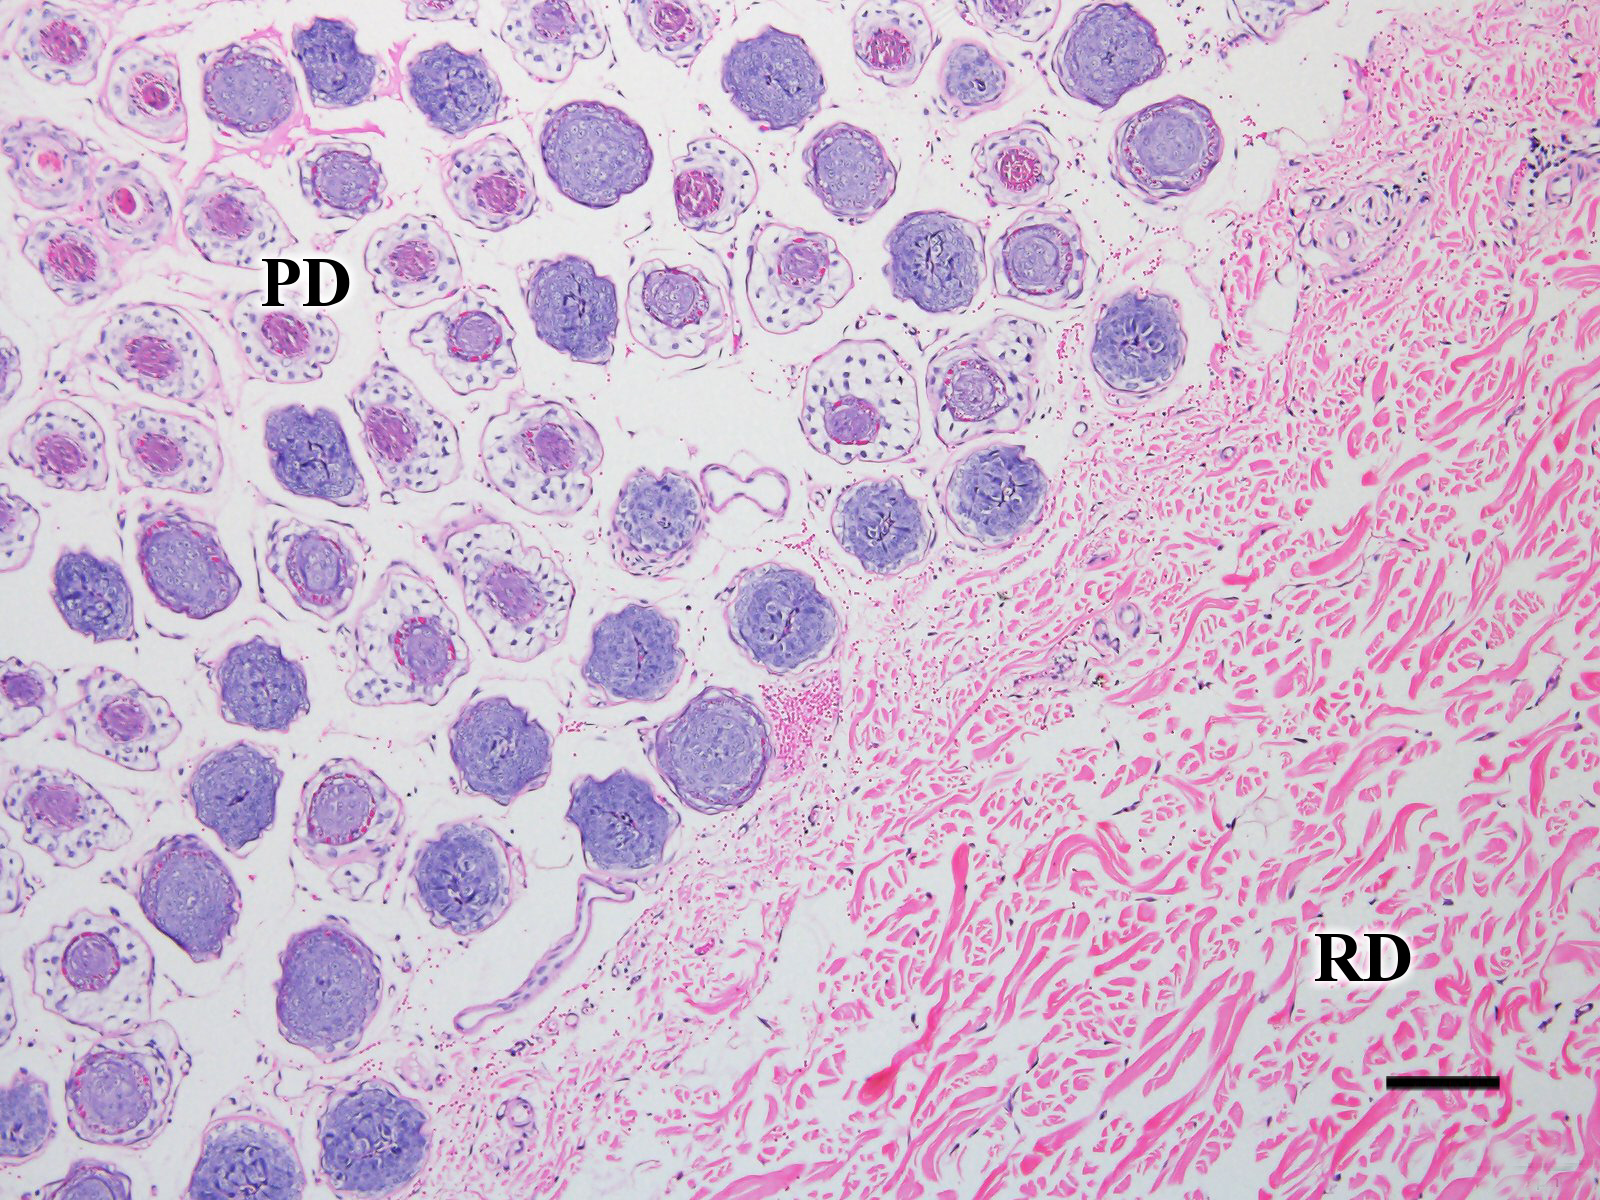
\includegraphics[width=0.7\textwidth]{fig8b.jpg}
  }
  \caption{Vertical sections from a wrinkled (a) and a wrinkle-free (b)  sheep from Trial 2 flock 1 stained with H-E, and viewed with a 10x objective. Skin layers are: {\bf PD} papillary dermis, and {\bf RD} reticular dermis. Scale bar is $80\mu m$.}
\vfill
  \label{fig:he10x}
\end{figure}

%\end{document}

